\documentclass[10pt]{article}
\textheight=9.25in \textwidth=7in \topmargin=-.75in
 \oddsidemargin=-0.25in
\evensidemargin=-0.25in
\usepackage{url}  % The bib file uses this
\usepackage{graphicx} %to import pictures
\usepackage{amsmath, amssymb}
\usepackage{theorem, multicol, color}
\usepackage{gfsartemisia-euler}
\usepackage{ulem}
\setlength{\intextsep}{5mm} \setlength{\textfloatsep}{5mm}
\setlength{\floatsep}{5mm}
\setlength{\parindent}{0em} % new paragraphs are not indented
\setcounter{MaxMatrixCols}{20}
\usepackage{caption}
\captionsetup[figure]{font=small}


%%%%  SHORTCUT COMMANDS  %%%%
\newcommand{\ds}{\displaystyle}
\newcommand{\Z}{\mathbb{Z}}
\newcommand{\arc}{\rightarrow}
\newcommand{\R}{\mathbb{R}}
\newcommand{\N}{\mathbb{N}}
\newcommand{\Q}{\mathbb{Q}}
\renewcommand{\P}{\mathbb{P}}
\newcommand{\blank}{\underline{\hspace{0.33in}}}
\newcommand{\qand}{\quad and \quad}
\renewcommand{\stirling}[2]{\genfrac{\{}{\}}{0pt}{}{#1}{#2}}
\newcommand{\dydx}{\ds \frac{d y}{d x}}
\newcommand{\ddx}{\ds \frac{d}{d x}}
\newcommand{\dvdx}{\ds \frac{d v}{d x}} 
\newcommand{\solution}{\color{blue} Solution: \color{black}}
%%%%  footnote style %%%%

\renewcommand{\thefootnote}{\fnsymbol{footnote}}

\pagestyle{empty}

\begin{document}

\begin{flushright}
Chandler Justice - A02313187
\end{flushright}
\noindent \underline{\hspace{3in}}\\
\textbf{CLASS:} Quiz \#4\\
\textbf{Due:} March 6, 2026 @ 23:59\\

	\begin{enumerate}
		\item Prove the following lemma.
		
            {\bf Lemma 1.} \emph{Every odd integer can be expressed as the difference of $2$ square \xout{positive} \textit{non-negative} integers.}
	
        \solution Observe the following sequence of square positive values:
        
        \begin{center}
            \begin{tabular}{|l|l|}
            $s_n$ & 01 ~ 04 ~ 09 ~ 16 ~ 25 ~ 36 ~ $\cdots$\\
            \hline
            $s_{n + 1} - s_n$ & ~ 03 ~ 05 ~ 07 ~ 09 ~ 11 ~ $\cdots$
            \end{tabular}
        \end{center}
        
        This hints that it isn't just the difference of two arbitrary squares, but two subsequent squares. Observe the following sequence $o_n$\footnote{$o$ for odd :)} for $n \geq 0$:

        \begin{align*}
            o_n &= (n + 1)^2 - n^2\\
                &= n^2 + 2n + 1 - n^2\\
                &= 2n + 1
        \end{align*}
        Then we can see $o_n = 2n + 1$ produces the sequence of odd positive integers. For any $n$, we can see the value will always be odd as it is some value with $2$ as a divisor which is then incremented by one, meaning the value no longer has $2$ as a divisor and is odd. Therefore, $o_n$ produces the sequence of odd integers. $\hfill\blacksquare$\\

		\item Use Lemma 1 to prove $$\sum_{k=1}^n (2k-1) = n^2.$$
		
            \solution We can see that this is a summation over every odd integer between $1$ and $n$. The sequence we obtain from lemma $1$ started at $0$, but we can see $o_{n-1} = n^2 - (n - 1)^2$ corrects the summation we found in problem 1 for the bounds of the summation. Observe
            \[\sum_{k=1}^n (2k - 1) = \sum_{k=1}^n [k^2 - (k-1)^2]\]
            We can see this creates a telescoping sum
            \begin{align*}
                \sum_{k=1}^n [k^2 - (k-1)^2] &= (1^2 - 0^2) + (2^2 - 1^2) + (3^2 - 2^2) + \cdots + (n^2 - (n-1)^2)\\
                                             &= n^2 - 0^2\\
                                             &= n^2
            \end{align*}
            Therefore, $LHS = RHS. \hfill\blacksquare$
            \newpage
		\item Use figureative- or polygonal-number reasoning and the figure below to derive a formula for $\ds\sum_{k=1}^n k^2$.
		
		
		\begin{center}
			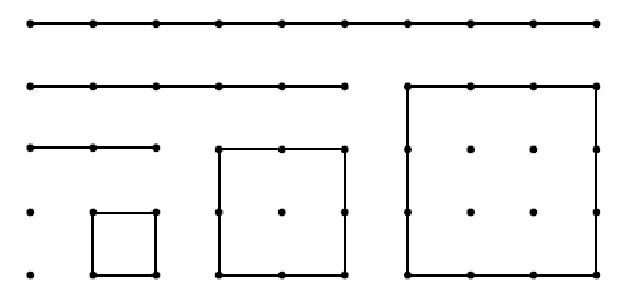
\includegraphics[scale=0.6]{sum_of_squares_suggestion.pdf}
		\end{center}

        \solution The lines give us the triangular numbers, while the squares give us the square numbers. We can see the number of square numbers is equal to the number of dots in the triangular number $t_n$ plus the triangular number $t_{n-1}$. We will denote the square numbers $s_n$. We can see $s_2  = 4 = t_2 + t_1 = 3 + 1$, $s_3 = 9 = t_3 + t_2 = 6 + 3$, $s_4 = 16 = t_4 + t_3 = 10 + 6$.\\

        Then we can see $\sum_{k=1}^n k^2 = \sum_{k=1}^n(t_n + t_{n-1})$. In class, we discussed the triangular numbers have the form $\frac{n(n+1)}{2}$ for all $n > 0$, and provided a proof of this formula. Observe
        \begin{align*}
            \sum_{k=1}^n k^2 &= \sum_{k=1}^n(t_n + t_{n-1})\\
                             &= \sum_{k=1}^n \frac{k(k+1)}{2} + \sum_{k=1}^n \frac{k(k-1)}{2}\\
                             &= \frac{1}{2}\sum_{k=1}^n k(k+1) + \frac{1}{2}\sum_{k=1}^n k(k-1)\\
        \end{align*}
        At this point, we employ discrete calculus to push us along to a closed from. Recall that \textit{falling factorials} have the form
        \[k^n = k(k-1)(k-2)\cdots(k-n+1)\]
        then we can see $k^{(2)} = k(k-1)$ and apply the antidifference of the summation of a falling power directly. Recall
    \[\sum_{k=1}^n k^{(r)} = \frac{(n+1)^{(r+1)}}{r+1}\]
    So the second summation has closed form
    \[\frac{1}{2}\sum_{k=1}^n k(k-1) = \frac{1}{2}\sum_{k=1}^n k^{(2)} = \frac{1}{2}\frac{(n + 1)^{(3)}}{3} = \frac{(n+1)(n)(n-1)}{6}\]
    Our first summation we need to manipulate a bit. Observe
    \[\frac{1}{2}\sum_{k=1}^n k(k+1) = \frac{1}{2} \sum_{k=1}^n (k^{(2)} + 2k) \]
    Then we can see our closed form is
    \[\frac{n(n-1)(n-2)}{6} + \frac{n(n-1)(n-2)}{6} + \frac{n(n-1)}{2}\]
    which simplifies to 
    \[\frac{n(n+1)(2n+1)}{6}\]
    the closed form of $n^3$.

        \item Let $t_n$ denote the $n^{\mbox{th}}$ triangular number ($t_1 = 1, t_2 = 3, t_4 = 6, \dots$) and $T_n$ denote $t_1 + t_2 + \cdots +t_n$ (these are sometimes called the \emph{tetrahedral numbers}).  Show that $\ds \sum_{k=1}^n k^2 = t_{n} + 2T_{n-1}$.
		
		\item Prove the Fundamental Theorem of Arithmetic using propositions from \emph{Euclid's Elements}. Use the propositions with impunity; you don't need to prove them. 
		
		{\bf The Fundamental Theorem of Arithmetic.} \emph{Every positive integer $n > 1$ can be expressed uniquely (disregarding their order) as the product of primes.}
		
		
	\end{enumerate}


\noindent \underline{\hspace{3in}}\\

\end{document}

